\documentclass[]{article}
\usepackage{mathtools,amssymb,amsthm,url,cancel,fancyhdr,graphicx,tensor}
\newtheorem{theorem}{Theorem}
\newtheorem{lemma}[theorem]{Lemma}
\newtheorem{corollary}[theorem]{Corollary}
\newcommand\numberthis{\addtocounter{equation}{1}\tag{\theequation}}
\fancyhead[L]{}
\fancyhead[C]{
	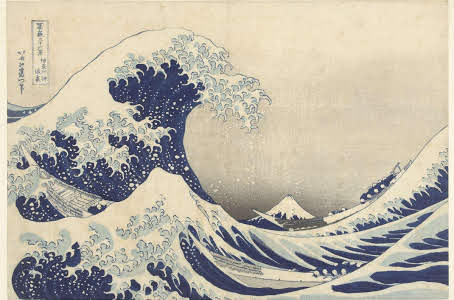
\includegraphics[width=6cm]{kanagawa.jpg}
}

\setlength\headheight{60pt} 

\graphicspath{ {images/} }

\pagestyle{plain}
% Title Page
\title{Introduction into General Relativity\\Assignment 9.2\\Gravitational Waves}
\author{Simon Crase}


\begin{document}
\maketitle
\thispagestyle{fancy}
\raggedright

\begin{theorem}\label{th:thethm}
Consider the metric tensor of the form: $g_{\mu\nu} \approx \eta_{\mu\nu} + h_{\mu\nu}$, where $|h_{\mu\nu}| \ll 1.$ Here $\eta_{\mu\nu}$ is the background Minkowskian metric tensor, while $h_{\mu\nu}$ is a small perturbation on top of it.

Then that the Riemann tensor has the following form at the linear order in $h_{\mu\nu}$:

\begin{align*}
R^{(1)}_{\mu\nu\alpha\beta} =& \eta_{\mu\gamma}\big[\partial_{\alpha}\Gamma^{\gamma}_{\nu\beta} - \partial_{\beta}\Gamma^{\gamma}_{\nu\alpha}\big]\numberthis\label{eq:R1}\\
\approx& \frac{1}{2}\big[\partial_{\nu}\partial_{\alpha}h_{\mu\beta} + \partial_{\mu}\partial_{\beta}h_{\nu\alpha} - \partial_{\mu}\partial_{\alpha}h_{\nu\beta} - \partial_{\nu}\partial_{\beta}h_{\mu\alpha}\big]\numberthis\label{eq:R2}
\end{align*}

Furthermore, in the gauge 
\begin{align*}
\partial_{\mu}(h^{\mu}_{\nu}-\frac{1}{2}\delta^{\mu}_{\nu}h)=&0\text{, the Ricci tensor is:}\\
R^{(1)}_{\mu\nu} =& - \frac{1}{2} \Box h_{\mu_{\nu}} \text{. where:}\\
\Box \triangleq & \eta^{\alpha\beta}\partial_{\alpha}\partial_{\beta}
\end{align*}
 
\end{theorem}

\begin{proof}
	We begin with a useful Lemma and Corollary.
	\begin{lemma}\label{lemma:gamma}
		For $g_{\mu\nu} \approx \eta_{\mu\nu} + h_{\mu\nu}$, where $|h_{\mu\nu}| \ll 1,  \Gamma^{\alpha}_{\mu\nu}$ is $\mathcal{O}(h)$, i.e., is of linear order in the $h_{\mu\nu}$ .
	\end{lemma}
    \begin{proof}[Proof of Lemma]
    	\begin{align*}
    	\text{	\cite[(46)]{akhmedev2016}}\implies&\\
    	\Gamma^{\alpha}_{\mu\nu} =& \frac{1}{2} \big(\eta^{\alpha\beta}+h^{\alpha\beta}\big)\big[\partial_{\nu}\big(\eta_{\beta\mu}+h_{\beta\mu}\big)+\partial_{\mu}\big(\eta_{\nu\beta}+h_{\nu\beta}\big)-\partial_{\beta}\big(\eta_{\mu\nu}+h_{\mu\nu}\big)\big] \\
    	=& \frac{1}{2} \big(\eta^{\alpha\beta}+h^{\alpha\beta}\big)\big[\partial_{\nu}h_{\beta\mu}+\partial_{\mu}h_{\nu\beta}-\partial_{\beta}h_{\mu\nu}\big]\\
    	=& \frac{1}{2} \eta^{\alpha\beta}\big[\partial_{\nu}h_{\beta\mu}+\partial_{\mu}h_{\nu\beta}-\partial_{\beta}h_{\mu\nu}\big] + \mathcal{O}(h^2)\\
    	=& \frac{1}{2} \big[\partial_{\nu}h^{\alpha}_{\mu}+\partial_{\mu}h^{\alpha}_{\nu}-\eta^{\alpha\beta}\partial_{\beta}h_{\mu\nu}\big] + \mathcal{O}(h^2) \numberthis\label{eq:Gamma} \\
    	=& \mathcal{O}(h)
    	\end{align*}
    \end{proof}
	\begin{corollary}\label{cor}
		With the same assumption, terms of the form $\Gamma^{.}_{..}\Gamma^{.}_{..}$ are $\mathcal{O}(h^2)$, and can be ignored.
	\end{corollary}
	Proof of Theorem \ref{th:thethm}.
	\begin{align*}
	\text{\cite[(53)]{akhmedev2016}}\implies&\\
	R\indices{^{\mu}_{\nu\alpha\beta}}=&\partial_{\alpha}\Gamma^{\mu}_{\nu\beta} - \partial_{\beta}\Gamma^{\mu}_{\nu\alpha} + \Gamma^{\mu}_{\gamma\alpha}\Gamma^{\nu}_{\mu\beta} - \Gamma^{\mu}_{\gamma\beta} \Gamma^{\gamma}_{\nu\alpha}\\
	=& \partial_{\alpha}\Gamma^{\mu}_{\nu\beta} - \partial_{\beta}\Gamma^{\mu}_{\nu\alpha} + \mathcal{O}(h^2)\text{, by Corollary \ref{cor}}\\
	R_{\mu\nu\alpha\beta} =&\big(\eta_{\mu\gamma}+h_{\mu\gamma}\big)	R\indices{^{\gamma}_{\nu\alpha\beta}}\\
	=&\big(\eta_{\mu\gamma}+h_{\mu\gamma}\big) \big(\partial_{\alpha}\Gamma^{\gamma}_{\nu\beta} - \partial_{\beta}\Gamma^{\gamma}_{\nu\alpha} + \mathcal{O}(h^2)\big)\\
	=&\eta_{\mu\gamma}\big(\partial_{\alpha}\Gamma^{\gamma}_{\nu\beta} - \partial_{\beta}\Gamma^{\gamma}_{\nu\alpha} \big)+ \mathcal{O}(h^2)\text{, in agreement with(\ref{eq:R1}).}
	\end{align*}
	We expand this expression using Lemma \ref{lemma:gamma} and (\ref{eq:Gamma}).
	\begin{align*}
	R_{\mu\nu\alpha\beta} =&\eta_{\mu\gamma}\big(\partial_{\alpha}\Gamma^{\gamma}_{\nu\beta} - \partial_{\beta}\Gamma^{\gamma}_{\nu\alpha} \big)+ \mathcal{O}(h^2)\\
	=&\frac{1}{2}\eta_{\mu\gamma}\big[\partial_{\alpha}\big( \partial_{\beta}h^{\gamma}_{\nu} + \partial_{\nu}h^{\gamma}_{\beta}-\partial^{\gamma}h_{\nu\beta}  \big) - \partial_{\beta}\big( \partial_{\alpha}h^{\gamma}_{\nu}+\partial_{\nu}h^{\gamma}_{\alpha}-\partial^{\gamma}h_{\nu\alpha}  \big)\big]+ \mathcal{O}(h^2)\\
	\approxeq&\frac{1}{2}\eta_{\mu\gamma}\big[\cancel{\partial_{\alpha}\partial_{\beta}h^{\gamma}_{\nu}} + \partial_{\alpha}\partial_{\nu}h^{\gamma}_{\beta}-\partial_{\alpha}\partial^{\gamma}h_{\nu\beta}  -  \cancel{\partial_{\beta}\partial_{\alpha}h^{\gamma}_{\nu}}-\partial_{\beta}\partial_{\nu}h^{\gamma}_{\alpha}+\partial_{\beta}\partial^{\gamma}h_{\nu\alpha}  \big]+ \mathcal{O}(h^2)\\
	\approxeq&\frac{1}{2}\eta_{\mu\gamma}\big[ \partial_{\alpha}\partial_{\nu}h^{\gamma}_{\beta}-\partial_{\alpha}\partial^{\gamma}h_{\nu\beta}  -\partial_{\beta}\partial_{\nu}h^{\gamma}_{\alpha}+\partial_{\beta}\partial^{\gamma}h_{\nu\alpha}  \big]+ \mathcal{O}(h^2)
	\\
	\approxeq&\frac{1}{2}\big[ \partial_{\alpha}\partial_{\nu}h_{\mu\beta}-\partial_{\alpha}\partial_{\mu}h_{\nu\beta}  -\partial_{\beta}\partial_{\nu}h_{\mu\alpha}+\partial_{\beta}\partial_{\mu}h_{\nu\alpha}  \big]+ \mathcal{O}(h^2)\\
	\approxeq&\frac{1}{2}\big[\partial_{\nu}\partial_{\alpha}h_{\mu\beta} + \partial_{\mu}\partial_{\beta}h_{\nu\alpha} - \partial_{\mu}\partial_{\alpha}h_{\nu\beta} - \partial_{\nu}\partial_{\beta}h_{\mu\alpha}\big]+ \mathcal{O}(h^2) \numberthis\label{eq:R}\\
	\text{using }& \partial_{\mu}\partial_{\beta}=\partial_{\beta}\partial_{\mu} \text{ etc, and rearranging terms.}
	\end{align*}
	This is the same as (\ref{eq:R2}).
\end{proof}

\begin{thebibliography}{9}
	
	\bibitem{akhmedev2016}
	Emil T. Akhmedev,
	\emph{Lectures on General Theory of Relativity},
	2016,
	\url{https://arxiv.org/pdf/1601.04996v6.pdf}.
	
	
\end{thebibliography}

\end{document}          
